\section{钳口三维建模}

\begin{figure}[htbp]
\centering
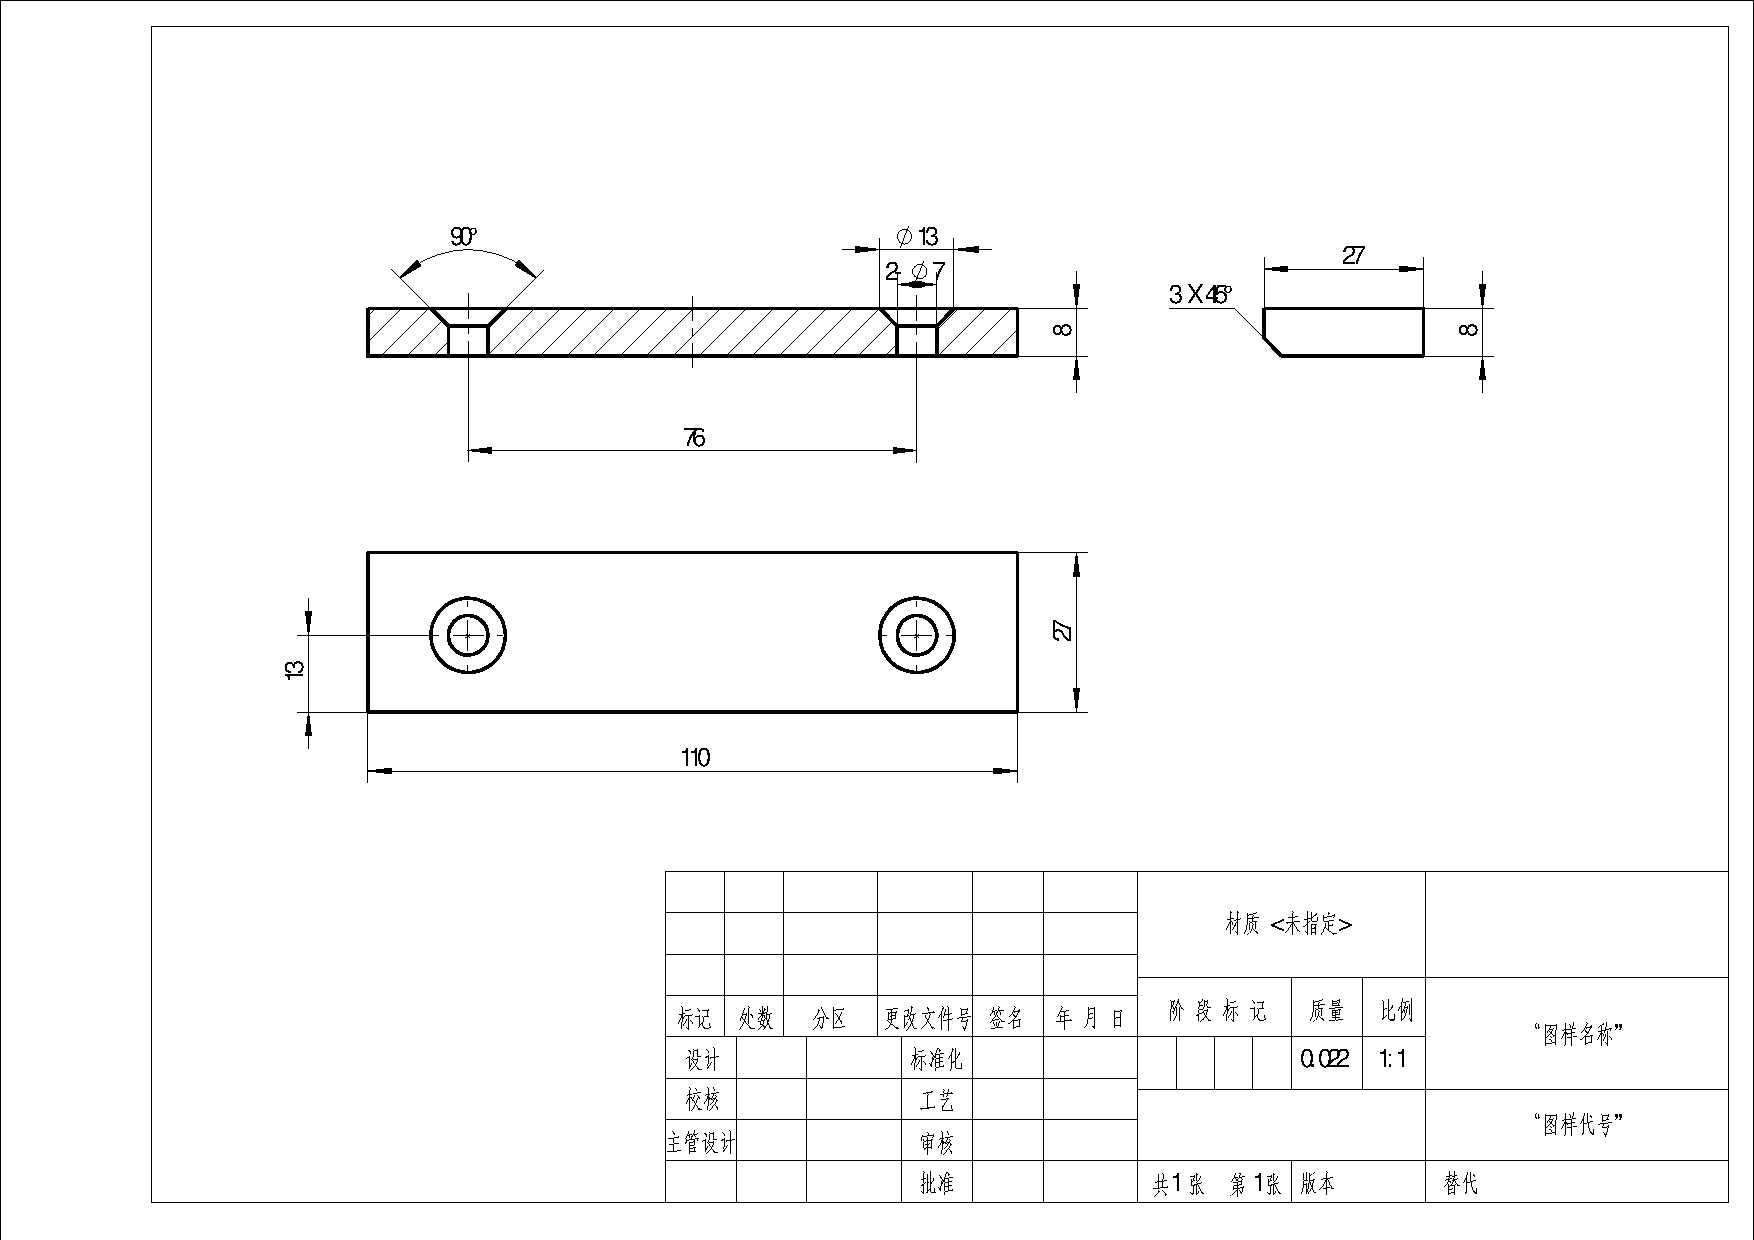
\includegraphics[width=0.8\textwidth]{taihuqianko.pdf}
\caption{钳口零件图}\label{fig:taihuqianko}
\end{figure}

在台虎钳的固定钳身和活动钳身上,均装有钢制钳口,并用螺钉固定。钳口的工作面上制有交叉的网纹,使工件夹紧后不易产生滑动。钳口经过热处理淬硬,具有较好的耐磨性。其具体的零件尺寸如图\ref{fig:taihuqianko}所示。

\begin{procedure}
\item 切换三维视图方向

打开AutoCAD后,将视图方向切换为西南等轴测。

\begin{lstlisting}
命令: -VIEW
输入选项 [?/删除(D)/正交(O)/恢复(R)/保存(S)/设置(E)/窗口(W)]: swiso
\end{lstlisting}

\item 构建钳口整体

从钳口零件图的可以看出,忽略钳口上的沉头孔后其整体是一块有倒角的板,补齐倒角切除部分的实体,则为一块形状为长方体的板。因此先绘制长方体作为构建钳口模型的基础,其结果如图\ref{fig:qiankoujianmo1} 所示。

\begin{lstlisting}
命令: BOX
指定第一个角点或 [中心(C)]:
指定其他角点或 [立方体(C)/长度(L)]: @110,27
指定高度或 [两点(2P)]: 8
\end{lstlisting}

\begin{figure}[htbp]
\centering
\begin{floatrow}[2]
\ffigbox{\caption{钳口基础长方体}\label{fig:qiankoujianmo1}}{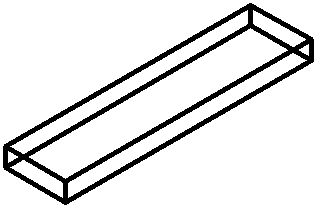
\includegraphics[width=0.4\textwidth]{qiankoujianmo1}}
\ffigbox{\caption{用户坐标系位置}\label{fig:qiankoujianmo2}}{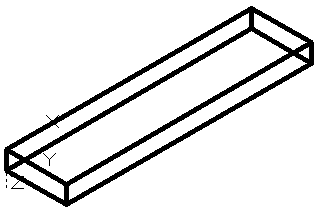
\includegraphics[width=.4\textwidth]{qiankoujianmo2}}
\end{floatrow}

\end{figure}

\item 构建沉头孔切除实体

为方便定位,我们先将用户坐标系定义到基础长方体之上。结果如图\ref{fig:qiankoujianmo2} 所示。

\begin{lstlisting}
命令: UCS
当前 UCS 名称: *世界*
指定 UCS 的原点或 [面(F)/命名(NA)/对象(OB)/上一个(P)/视图(V)/世界(W)/X/Y/Z/Z 轴(ZA)] <世界>:
指定 X 轴上的点或 <接受>:
指定 XY 平面上的点或 <接受>:
\end{lstlisting}

由于沉头孔是在长方体的基础上切除了一个母线夹角$90^o$的圆锥台和一个直径为$\phi 7$的圆柱体。圆锥台和圆锥体都属于回转体类基本几何体。图\ref{fig:yuanzhutix} 为圆锥体的实体模型和投影视图。从投影图中可以看出圆锥体的底面与水平投影面平行,其投影为一圆,反映圆锥底面的实形,在其余两个投影面上圆锥底面的投影积聚为一条直线;圆锥体的其余两面投影均为等腰三角形。圆锥体是顶圆半径为零的圆锥台。

\begin{figure}[htbp]
\centering
\subfloat[]{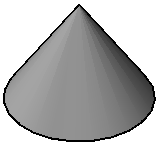
\includegraphics[scale=1]{yuanzhuiti.png}}\hspace{30pt}
\subfloat[]{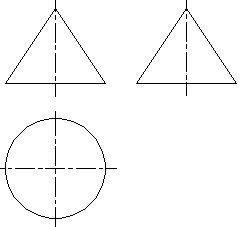
\includegraphics[scale=0.7]{yuanzhuitithreeview.png}}
\caption{圆锥体的投影}\label{fig:yuanzhuiti}
\end{figure}

在AutoCAD中构建圆锥台实体需要用到圆锥体命令,其调用方法有:
\begin{itemize}
\item 键盘输入cone\index{cone,圆锥体}
\item 【绘图】$\rightarrow $【建模】$\rightarrow $【圆锥体】
\item 【实体】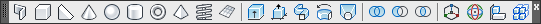
\includegraphics[scale=0.45]{solidtoolbar}工具栏中的【圆锥体】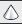
\includegraphics[scale=0.5]{conetool}图标
\end{itemize}

命令调用后要示指定圆锥体的底面中心位置,根据钳口零件图计算可知,沉头孔的圆锥台的圆心坐标是(17,14),故以此绝对坐标值指定其圆心。

\begin{lstlisting}
命令: CONE
指定底面的中心点或 [三点(3P)/两点(2P)/切点、切点、半径(T)/椭圆(E)]: 17,14
\end{lstlisting}

接下来根据命令提示,以值6.5作为底面半径。

\begin{lstlisting}
指定底面半径或 [直径(D)] <16.4173>: 6.5
\end{lstlisting}

由于AutoCAD默认是绘制圆锥体,要绘制圆锥台就需要选择【顶面半径(T)】选项来指定顶面半径。

\begin{lstlisting}
指定高度或 [两点(2P)/轴端点(A)/顶面半径(T)] <8.0000>: t
\end{lstlisting}

接下来以值3.5作为顶面的半径。

\begin{lstlisting}
指定顶面半径 <8.0000>: 3.5
\end{lstlisting}

最后指定圆锥台的高底,经过简单的计算可知其高度值为1.5,构建圆锥台的结果如图\ref{fig:qiankoujianmo3}所示。

\begin{lstlisting}
指定高度或 [两点(2P)/轴端点(A)] <8.0000>: 1.5
\end{lstlisting}

\begin{figure}[htbp]
\centering
\begin{floatrow}[2]
\ffigbox{\caption{构建圆锥台}\label{fig:qiankoujianmo3}}{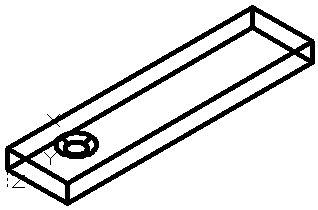
\includegraphics[width=0.4\textwidth]{qiankoujianmo3}}
\ffigbox{\caption{添加圆柱体}\label{fig:qiankoujianmo4}}{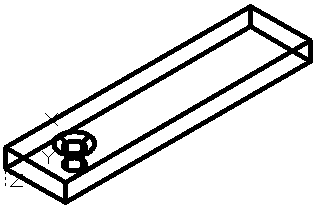
\includegraphics[width=0.4\textwidth]{qiankoujianmo4}}
\end{floatrow}
\end{figure}

完成圆锥台的构建后,以其顶面圆心作为圆体的圆心构建沉头孔切除实体中的圆柱体,结果如图\ref{fig:qiankoujianmo4}所示。

\begin{lstlisting}
命令: CYLINDER
指定底面的中心点或 [三点(3P)/两点(2P)/切点、切点、半径(T)/椭圆(E)]:
指定底面半径或 [直径(D)] <6.5000>: 3.5
指定高度或 [两点(2P)/轴端点(A)] <1.5000>: 6.5
\end{lstlisting}

为方便后后续的三维镜像操作和差集操作,因此将圆锥台和圆体合并为一个实体。

\begin{lstlisting}
命令: UNION
选择对象: 找到 1 个
选择对象: 找到 1 个,总计 2 个
选择对象:
\end{lstlisting}

\item 镜像沉头孔切除实体

由于钳口零件中的两个沉头孔是对称的,因此可以用三维镜像命令来实现第二个沉头孔切除实体。图\ref{fig:qiankoujianmo5}是三维镜像后的结果。

\begin{lstlisting}
命令: MIRROR3D
选择对象: 找到 1 个
选择对象:
指定镜像平面 (三点) 的第一个点或
  [对象(O)/最近的(L)/Z 轴(Z)/视图(V)/XY 平面(XY)/YZ 平面(YZ)/ZX 平面(ZX)/三点(3)] <三点>: 
  在镜像平面上指定第二点: 
  在镜像平面上指定第三点:
是否删除源对象?[是(Y)/否(N)] <否>:
\end{lstlisting}

\begin{figure}[htbp]
\centering
\begin{floatrow}[2]
\ffigbox{\caption{镜像切除实体}\label{fig:qiankoujianmo5}}{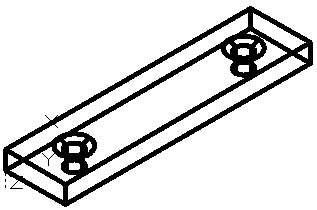
\includegraphics[width=0.4\textwidth]{qiankoujianmo5}}
\ffigbox{\caption{制作倒角边}\label{fig:qiankoujianmo6}}{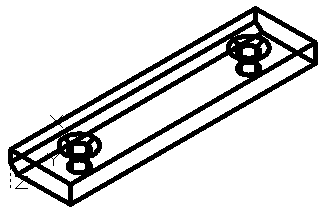
\includegraphics[width=0.4\textwidth]{qiankoujianmo6}}
\end{floatrow}
\end{figure}

\item 构建沉头孔

完成沉头孔实体的制作后,还需要将其从钳口基础长方体中去除才能够真正的构建沉头孔,故用差集来完成此项操作。
\begin{lstlisting}
命令: SUBTRACT
选择要从中减去的实体、曲面和面域...
选择对象: 找到 1 个
选择对象:  选择要减去的实体、曲面和面域...
选择对象: 找到 1 个
选择对象: 找到 1 个,总计 2 个
选择对象:
\end{lstlisting}

\item 倒角边

至此,还剩下一条角边没有完。在钳口零件图中,倒角边的尺寸是以$3\times 45^o$的形式来表示的,其含义是倒角边斜面与夹角为45度,直角边距离为3mm。根据该尺寸可知倒角边能够完成倒角边命令的构建,结果如图\ref{fig:qiankoujianmo6}所示。

\begin{lstlisting}
命令:
CHAMFEREDGE
距离 1 = 1.0000,距离 2 = 1.0000
选择一条边或 [环(L)/距离(D)]: d
指定距离 1 或 [表达式(E)] <1.0000>: 3
指定距离 2 或 [表达式(E)] <1.0000>: 3
选择一条边或 [环(L)/距离(D)]:
选择同一个面上的其他边或 [环(L)/距离(D)]:
按 Enter 键接受倒角或 [距离(D)]:
\end{lstlisting}

\item 切换视觉样式

为使钳口零件更具立体感,我们将视觉样式从二维线框模式切换为灰度,其结果如图\ref{fig:qiankoujianmo7}所示 。


\begin{figure}[htbp]
\centering
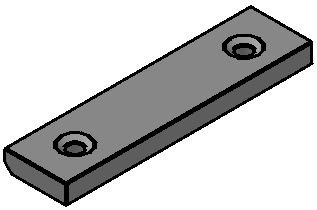
\includegraphics[width=0.5\textwidth]{qiankoujianmo7}
\caption{钳口三维模型}\label{fig:qiankoujianmo7}
\end{figure}
\begin{lstlisting}
命令: vscurrent
输入选项 [二维线框(2)/线框(W)/隐藏(H)/真实(R)/概念(C)/着色(S)/带边缘着色(E)/灰度(G)/勾画(SK)/X 射线(X)/其他(O)] <二维线框>: g
\end{lstlisting}

\item 保存模型

最后将构建好的钳口三维模型以文件名“钳口.dwg”进行保存。
\end{procedure}
\endinput